% Nuran — Talk & Learn · User Manual
% XeLaTeX, Poppins display + Lato text, TikZ screen mockups in the app's own palette.
\documentclass[10.5pt]{article}
\usepackage[letterpaper,top=2.2cm,bottom=2.4cm,left=2.3cm,right=2.3cm]{geometry}
\usepackage{fontspec}
\setmainfont{Lato}
\newfontfamily\disp{Poppins}
\newfontfamily\dispmed{Poppins Medium}
\usepackage{xcolor}
\definecolor{cream}{HTML}{F7F4EE}
\definecolor{surface}{HTML}{FFFDF8}
\definecolor{ink}{HTML}{2F3A43}
\definecolor{inksoft}{HTML}{55636E}
\definecolor{linec}{HTML}{D8D2C6}
\definecolor{green}{HTML}{E2EBDE}\definecolor{greenE}{HTML}{82A077}
\definecolor{yellow}{HTML}{F3ECD4}\definecolor{yellowE}{HTML}{B3A266}
\definecolor{rose}{HTML}{F1E0E4}\definecolor{roseE}{HTML}{B3808F}
\definecolor{blue}{HTML}{DFE9EF}\definecolor{blueE}{HTML}{7D9CB0}
\definecolor{peach}{HTML}{F3E5D8}\definecolor{peachE}{HTML}{B98F6B}
\definecolor{lav}{HTML}{E8E2F0}\definecolor{lavE}{HTML}{9384B5}
\definecolor{sage}{HTML}{E6ECE9}\definecolor{sageE}{HTML}{7FA093}
\definecolor{neut}{HTML}{EFECE5}\definecolor{neutE}{HTML}{9A9484}
\usepackage{tikz}
\usetikzlibrary{calc}
\usepackage[most]{tcolorbox}
\usepackage{tabularx}
\usepackage{booktabs}
\usepackage{enumitem}
\usepackage{fancyhdr}
\usepackage{graphicx}
\usepackage[hidelinks]{hyperref}
\color{ink}
\setlength{\parindent}{0pt}
\setlength{\parskip}{5pt}
\linespread{1.18}

% ---------- header/footer ----------
\pagestyle{fancy}
\fancyhf{}
\renewcommand{\headrulewidth}{0pt}
\fancyfoot[L]{\color{inksoft}\footnotesize Nuran — Talk \& Learn~~·~~User Manual}
\fancyfoot[R]{\color{inksoft}\footnotesize\thepage}
\fancyfoot[C]{}

% ---------- section heading ----------
\newcounter{sect}
\newcommand{\sect}[1]{%
  \stepcounter{sect}%
  \par\vspace{14pt}%
  {\noindent
\begin{tikzpicture}[baseline=(n.base)]
    \node[circle,fill=ink,text=cream,inner sep=0pt,minimum size=17pt,font=\disp\small] (n) {\thesect};
  \end{tikzpicture}\hspace{7pt}{\disp\large #1}}%
  \par\nopagebreak\vspace{2pt}\nopagebreak{\color{linec}\rule{\textwidth}{0.8pt}}\par\nopagebreak\vspace{6pt}}

\newcommand{\sub}[1]{\par\vspace{7pt}{\dispmed\small #1}\par\vspace{1pt}}

% ---------- callout number ----------
\newcommand{\co}[1]{\tikz[baseline=-0.62ex]{\node[circle,fill=ink,text=cream,inner sep=0.5pt,minimum size=11.5pt,font=\bfseries\scriptsize]{#1};}}

% ---------- tip box ----------
\newtcolorbox{tip}[1][Tip]{enhanced,breakable,frame hidden,boxrule=0pt,
  colback=blue!55!white,borderline west={2.5pt}{0pt}{blueE},
  left=9pt,right=9pt,top=6pt,bottom=6pt,arc=2pt,
  title={\dispmed\small #1},coltitle=ink,attach title to upper={\par}}
\newtcolorbox{warn}[1][Good to know]{enhanced,breakable,frame hidden,boxrule=0pt,
  colback=rose!55!white,borderline west={2.5pt}{0pt}{roseE},
  left=9pt,right=9pt,top=6pt,bottom=6pt,arc=2pt,
  title={\dispmed\small #1},coltitle=ink,attach title to upper={\par}}

% ---------- mockup pieces ----------
\tikzset{
  tileS/.style 2 args={rounded corners=7pt,draw=#1,fill=#2,line width=1.4pt},
  chipS/.style 2 args={rounded corners=5pt,draw=#1,fill=#2,line width=1.1pt},
  sym/.style={draw=ink!80!black,line width=1.5pt,line cap=round,line join=round},
  lbl/.style={font=\dispmed\small,text=ink},
  lblbig/.style={font=\dispmed\normalsize,text=ink},
  lblsm/.style={font=\dispmed\tiny,text=ink},
  ghost/.style={font=\small,text=inksoft},
}
% simple symbol pics (faithful to the app's SVG set)
\tikzset{
  yes/.pic={\draw[sym,fill=green] (0,0) circle (0.30);\draw[sym] (-0.13,-0.02) -- (-0.03,-0.12) -- (0.15,0.10);},
  no/.pic={\draw[sym,fill=rose] (0,0) circle (0.30);\draw[sym] (-0.11,-0.11) -- (0.11,0.11);\draw[sym] (-0.11,0.11) -- (0.11,-0.11);},
  person/.pic={\draw[sym,fill=yellow] (0,0.13) circle (0.105);\draw[sym,fill=yellow] (-0.13,-0.28) .. controls (-0.13,-0.02) .. (0,-0.02) .. controls (0.13,-0.02) .. (0.13,-0.28) -- cycle;},
  iarrow/.pic={\pic at (0.07,0) {person};\draw[sym,<-] (-0.06,-0.05) -- (-0.30,-0.02);},
  youarrow/.pic={\pic at (-0.07,0) {person};\draw[sym,->] (0.30,-0.02) -- (0.06,-0.05);},
  apple/.pic={\draw[sym,fill=rose] (0,-0.05) ellipse (0.24 and 0.22);\draw[sym] (0,0.17) .. controls (0.02,0.26) .. (0.10,0.30);},
  smiley/.pic={\draw[sym,fill=yellow] (0,0) circle (0.28);\fill[ink] (-0.10,0.06) circle (0.030);\fill[ink] (0.10,0.06) circle (0.030);\draw[sym] (-0.12,-0.08) .. controls (0,-0.18) .. (0.12,-0.08);},
  goarrow/.pic={\draw[sym,fill=green] (0,0) circle (0.28);\draw[sym,->] (-0.13,0) -- (0.14,0);},
  house/.pic={\draw[sym,fill=peach] (-0.20,-0.24) rectangle (0.20,0.06);\draw[sym] (-0.26,0.04) -- (0,0.26) -- (0.26,0.04);\draw[sym,fill=surface] (-0.05,-0.24) rectangle (0.06,-0.08);},
  ball/.pic={\draw[sym,fill=rose] (0,0) circle (0.27);\draw[sym] (-0.22,0.10) .. controls (0,0.0) .. (0.22,0.10);\draw[sym] (-0.22,-0.10) .. controls (0,0.0) .. (0.22,-0.10);},
  bubble/.pic={\draw[sym,fill=green,rounded corners=3.5pt] (-0.27,-0.10) rectangle (0.27,0.24);\draw[sym,fill=green] (-0.12,-0.095) -- (-0.03,-0.095) -- (-0.12,-0.22) -- cycle;\fill[ink] (-0.11,0.07) circle (0.025);\fill[ink] (0,0.07) circle (0.025);\fill[ink] (0.11,0.07) circle (0.025);},
  twopeople/.pic={\pic at (-0.09,0.02) {person};\pic[scale=0.8] at (0.16,-0.06) {person};},
  bell/.pic={\draw[sym,fill=rose] (-0.16,-0.10) .. controls (-0.16,0.22) .. (0,0.22) .. controls (0.16,0.22) .. (0.16,-0.10) -- (0.22,-0.16) -- (-0.22,-0.16) -- cycle;\draw[sym] (-0.05,-0.24) .. controls (0,-0.28) .. (0.05,-0.24);},
  star/.pic={\draw[sym,fill=yellow] (90:0.29) -- (162:0.13) -- (234:0.29) -- (275:0.12) -- (306:0.29) -- (350:0.13) -- (18:0.29) -- (54:0.13) -- cycle;},
  bodyheart/.pic={\pic at (-0.06,0) {person};\draw[sym,fill=rose] (0.20,0.16) .. controls (0.12,0.24) and (0.14,0.34) .. (0.22,0.30) .. controls (0.30,0.34) and (0.32,0.24) .. (0.24,0.16) .. controls (0.23,0.15) and (0.21,0.15) .. (0.20,0.16);},
}

\begin{document}

% ================= COVER =================
\thispagestyle{empty}
\begin{tikzpicture}[remember picture,overlay]
  \fill[cream] (current page.south west) rectangle (current page.north east);
  \foreach \x/\y/\p/\s in {2.7/-3.6/bubble/1.9, 18.4/-4.8/star/1.6, 3.1/-21.8/ball/1.8, 18.1/-20.6/apple/1.9}{
    \begin{scope}[opacity=0.45,shift={($(current page.north west)+(\x,\y)$)},scale=\s]
      \pic {\p};
    \end{scope}}
\end{tikzpicture}
\vspace*{3.2cm}
\begin{center}
  
\includegraphics[width=3.7cm]{icon-512.png}\\[26pt]
  {\disp\fontsize{30}{34}\selectfont Nuran}\\[6pt]
  {\dispmed\large Talk \& Learn}\\[26pt]
  {\color{inksoft}\rule{2.1cm}{0.8pt}}\\[26pt]
  {\disp\Large User Manual}\\[10pt]
  {\color{inksoft}\normalsize For parents, caregivers, and everyone who helps}\\[64pt]
  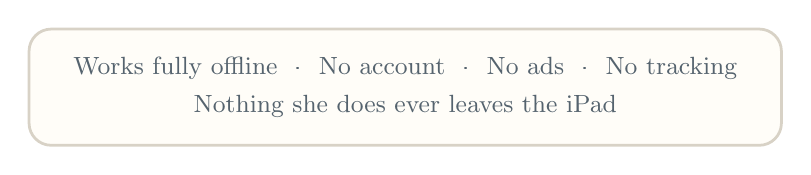
\begin{tikzpicture}
    \node[rounded corners=8pt,fill=surface,draw=linec,line width=1pt,inner xsep=16pt,inner ysep=10pt,align=center]
    {\color{inksoft}\small Works fully offline~~·~~No account~~·~~No ads~~·~~No tracking\\[2pt]
     \color{inksoft}\small Nothing she does ever leaves the iPad};
  \end{tikzpicture}
\end{center}
\vfill
\begin{center}{\color{inksoft}\footnotesize Version 1~~·~~2026~~·~~Free \& open source (MIT)}\end{center}
\newpage

% ================= WELCOME + TOC =================
{\disp\LARGE Welcome}\par\vspace{4pt}
{\color{linec}\rule{\textwidth}{0.8pt}}\par\vspace{8pt}

Nuran is a talking app for a child who communicates by pointing. She taps large picture
buttons and the iPad speaks each word slowly and clearly. You can add her own words with
your photos, put the family in with real faces and your recorded voice, and keep everything
safely backed up.

Two promises shape everything in this manual:

\begin{itemize}[leftmargin=16pt,itemsep=2pt]
  \item \textbf{She cannot break it.} Deleting is never permanent, settings live behind a
        caregiver gate, and the app heals itself if the iPad misbehaves.
  \item \textbf{It is completely private.} No account, no internet needed, no tracking.
        The only way any data leaves the iPad is if you personally export a backup file.
\end{itemize}

\vspace{10pt}
{\disp\LARGE Contents}\par\vspace{4pt}
{\color{linec}\rule{\textwidth}{0.8pt}}\par\vspace{10pt}

\newcommand{\tocrow}[3]{%
  \begin{tikzpicture}[baseline]
    \node[circle,fill=#3,draw=ink!30,inner sep=0pt,minimum size=15pt,font=\dispmed\scriptsize,text=ink] {#1};
  \end{tikzpicture}~~{\dispmed #2}\par\vspace{5.5pt}}
\begin{minipage}[t]{0.48\textwidth}
  \tocrow{1}{The home screen}{green}
  \tocrow{2}{Talking: words \& sentences}{yellow}
  \tocrow{3}{People \& the Help button}{rose}
  \tocrow{4}{The caregiver area}{blue}
\end{minipage}\hfill
\begin{minipage}[t]{0.48\textwidth}
  \tocrow{5}{Adding words \& people}{peach}
  \tocrow{6}{Settings}{lav}
  \tocrow{7}{Keeping everything safe}{sage}
  \tocrow{8}{Fixes \& helping her learn}{neut}
\end{minipage}

\vspace{14pt}
\begin{tip}[Two-minute quick start]
Open the app from its Home Screen icon, tap \textbf{Talk}, and tap any word — the iPad
speaks it. That is the whole idea. Everything else in this manual just makes that richer.
\end{tip}
\newpage

% ================= 1 HOME =================
\sect{The home screen}

Four large buttons and nothing else. The same four things are always in the same place,
which matters more than it looks: predictability is what makes the app feel safe to her.

\vspace{6pt}
\begin{center}
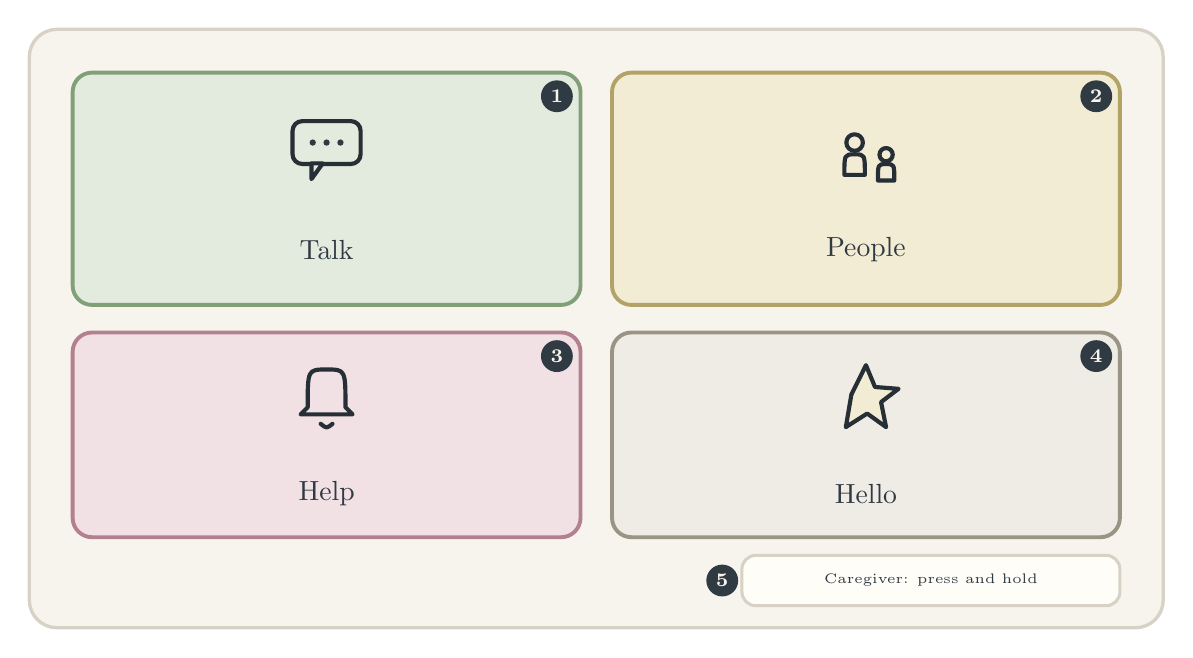
\begin{tikzpicture}[x=1cm,y=1cm]
  % frame
  \draw[rounded corners=10pt,fill=cream,draw=linec,line width=1.2pt] (0,0) rectangle (14.4,7.6);
  % tiles
  \draw[tileS={greenE}{green}]   (0.55,4.10) rectangle (7.00,7.05);
  \pic[scale=1.6] at (3.775,6.05) {bubble};  \node[lblbig] at (3.775,4.80) {Talk};
  \draw[tileS={yellowE}{yellow}] (7.40,4.10) rectangle (13.85,7.05);
  \pic[scale=1.6] at (10.625,6.0) {twopeople}; \node[lblbig] at (10.625,4.80) {People};
  \draw[tileS={roseE}{rose}]     (0.55,1.15) rectangle (7.00,3.75);
  \pic[scale=1.5] at (3.775,2.95) {bell};   \node[lblbig] at (3.775,1.70) {Help};
  \draw[tileS={neutE}{neut}]     (7.40,1.15) rectangle (13.85,3.75);
  \pic[scale=1.5] at (10.625,2.90) {star};  \node[lblbig] at (10.625,1.70) {Hello};
  % gate
  \draw[chipS={linec}{surface}] (9.05,0.28) rectangle (13.85,0.92);
  \node[lblsm] at (11.45,0.60) {Caregiver: press and hold};
  % callouts
  \node at (6.70,6.75) {\co{1}}; \node at (13.55,6.75) {\co{2}};
  \node at (6.70,3.45) {\co{3}}; \node at (13.55,3.45) {\co{4}};
  \node at (8.80,0.60) {\co{5}};
\end{tikzpicture}
\end{center}
\vspace{4pt}

\begin{description}[leftmargin=26pt,labelwidth=18pt,itemsep=3pt,font=\normalfont]
  \item[\co{1}] \textbf{Talk} opens the word buttons — where she communicates and learns. (Section 2)
  \item[\co{2}] \textbf{People} shows family photos that speak their names when tapped. (Section 3)
  \item[\co{3}] \textbf{Help} rings a loud alarm so she can call a caregiver from another room.
        Only an adult can silence it. (Section 3)
  \item[\co{4}] \textbf{Hello} simply says ``hello'' — a safe, friendly button to experiment with.
  \item[\co{5}] \textbf{Caregiver: press and hold.} Hold for about three seconds to open the
        caregiver area. A quick tap does nothing, so she cannot wander in by accident. (Section 4)
\end{description}
\newpage

% ================= 2 TALK =================
\sect{Talking: words \& sentences}

Tap a word, hear the word — spoken slowly, the way a speech therapist models it.
Around that simple idea sit four helpers, all visible on every Talk screen:

\vspace{6pt}
\begin{center}
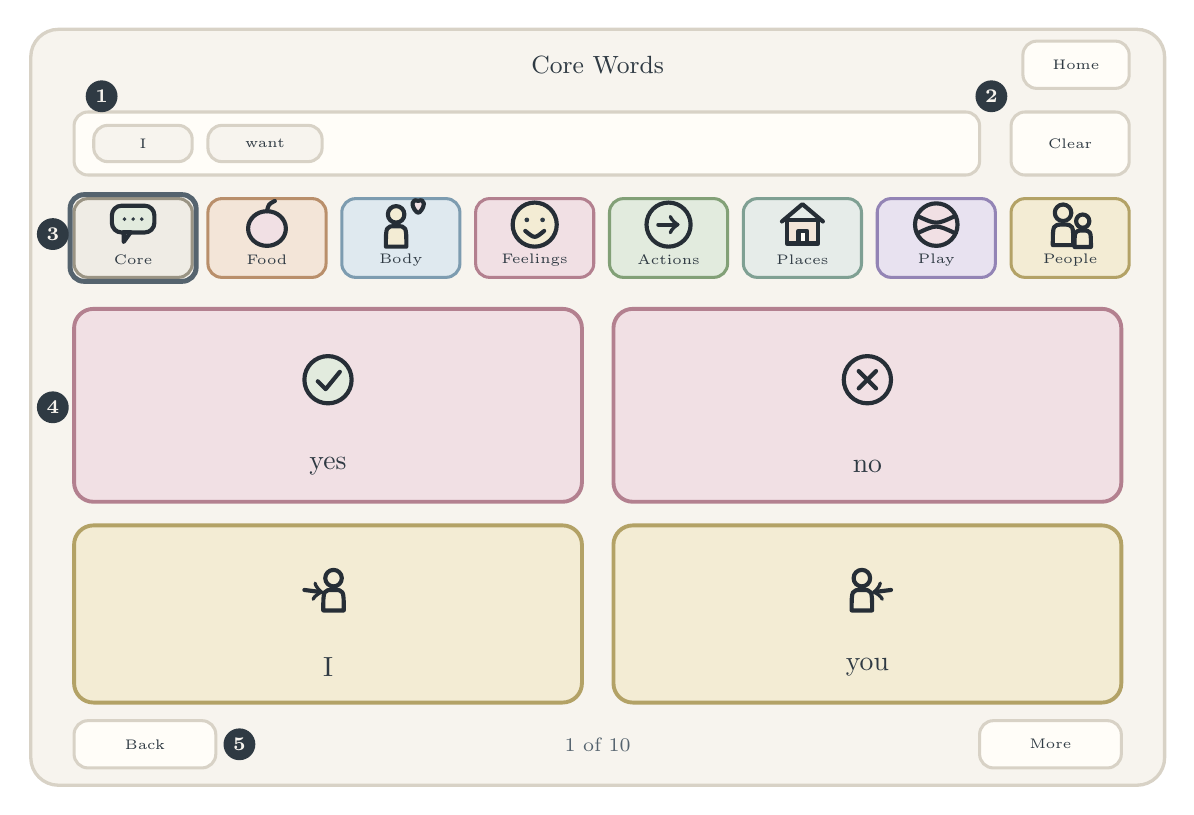
\begin{tikzpicture}[x=1cm,y=1cm]
  \draw[rounded corners=10pt,fill=cream,draw=linec,line width=1.2pt] (0,0) rectangle (14.4,9.6);
  % title row
  \node[lbl] at (7.2,9.15) {Core Words};
  \draw[chipS={linec}{surface}] (12.6,8.85) rectangle (13.95,9.45); \node[lblsm] at (13.275,9.15) {Home};
  % sentence bar
  \draw[chipS={linec}{surface}] (0.55,7.75) rectangle (12.05,8.55);
  \draw[chipS={linec}{cream}] (0.80,7.92) rectangle (2.05,8.38); \node[lblsm] at (1.425,8.15) {I};
  \draw[chipS={linec}{cream}] (2.25,7.92) rectangle (3.70,8.38); \node[lblsm] at (2.975,8.15) {want};
  \draw[chipS={linec}{surface}] (12.45,7.75) rectangle (13.95,8.55); \node[lblsm] at (13.20,8.15) {Clear};
  % group strip
  \foreach \i/\nm/\f/\e/\p in {0/Core/neut/neutE/bubble, 1/Food/peach/peachE/apple, 2/Body/blue/blueE/bodyheart, 3/Feelings/rose/roseE/smiley, 4/Actions/green/greenE/goarrow, 5/Places/sage/sageE/house, 6/Play/lav/lavE/ball, 7/People/yellow/yellowE/twopeople}{
    \draw[chipS={\e}{\f}] ($(0.55,6.45)+(\i*1.7,0)$) rectangle ($(2.05,7.45)+(\i*1.7,0)$);
    \begin{scope}[shift={($(1.30,7.12)+(\i*1.7,0)$)},scale=0.62]\pic {\p};\end{scope}
    \node[lblsm] at ($(1.30,6.67)+(\i*1.7,0)$) {\nm};}
  \draw[rounded corners=5pt,draw=inksoft,line width=1.8pt] (0.50,6.40) rectangle (2.10,7.50);
  % word tiles
  \draw[tileS={roseE}{rose}] (0.55,3.60) rectangle (7.00,6.05);
  \begin{scope}[shift={(3.775,5.15)},scale=1.25]\pic {yes};\end{scope} \node[lblbig] at (3.775,4.05) {yes};
  \draw[tileS={roseE}{rose}] (7.40,3.60) rectangle (13.85,6.05);
  \begin{scope}[shift={(10.625,5.15)},scale=1.25]\pic {no};\end{scope} \node[lblbig] at (10.625,4.05) {no};
  \draw[tileS={yellowE}{yellow}] (0.55,1.05) rectangle (7.00,3.30);
  \begin{scope}[shift={(3.775,2.50)},scale=1.25]\pic {iarrow};\end{scope} \node[lblbig] at (3.775,1.50) {I};
  \draw[tileS={yellowE}{yellow}] (7.40,1.05) rectangle (13.85,3.30);
  \begin{scope}[shift={(10.625,2.50)},scale=1.25]\pic {youarrow};\end{scope} \node[lblbig] at (10.625,1.50) {you};
  % pager
  \draw[chipS={linec}{surface}] (0.55,0.22) rectangle (2.35,0.82); \node[lblsm] at (1.45,0.52) {Back};
  \node[ghost,font=\scriptsize] at (7.2,0.52) {1 of 10};
  \draw[chipS={linec}{surface}] (12.05,0.22) rectangle (13.85,0.82); \node[lblsm] at (12.95,0.52) {More};
  % callouts
  \node at (0.90,8.75) {\co{1}}; \node at (12.20,8.75) {\co{2}};
  \node at (0.28,7.00) {\co{3}}; \node at (0.28,4.80) {\co{4}}; \node at (2.65,0.52) {\co{5}};
\end{tikzpicture}
\end{center}
\vspace{4pt}

\begin{description}[leftmargin=26pt,labelwidth=18pt,itemsep=3pt,font=\normalfont]
  \item[\co{1}] \textbf{The sentence bar.} Every tapped word also lands here, in order.
        Tap the bar itself and the iPad speaks the whole line — \emph{``I want cookie.''}
        It holds up to eight words and follows her across groups, so a sentence can start
        in Core Words and finish in Food \& Drink.
  \item[\co{2}] \textbf{Save / Clear.} Clear empties the bar. \emph{Holding} Save for a
        moment turns the sentence into a single button in a \textbf{My Phrases} group —
        so \emph{``I need the bathroom''} becomes one tap forever after. (Holding, not
        tapping, so stray taps cannot create buttons.)
  \item[\co{3}] \textbf{The group strip.} One colored button per word group; the group she
        is in has the darker outline. She moves between groups herself — no caregiver needed.
  \item[\co{4}] \textbf{Word buttons.} Picture and written word together, color-coded by
        type: people words yellow, actions green, feelings pink. Words you add appear here too.
  \item[\co{5}] \textbf{Back / More} turn pages when a group holds more words than one screen.
\end{description}

\begin{tip}
Colors are consistent everywhere: a word keeps its color across screens, so her hands
learn where things are before her reading does.
\end{tip}
\newpage

% ================= 3 PEOPLE & HELP =================
\sect{People \& the Help button}

\sub{People}
People shows the family as large photo tiles — real faces work far better than symbols
for social words. Tapping a photo speaks the person's name, in your recorded voice if you
added one, and the name joins the sentence bar just like a word: \emph{``I want mom.''}
A \textbf{Back to words} button returns her to Talk. People starts empty; adding the
family takes about a minute per person (Section 5).

\sub{The Help alarm}
When she taps \textbf{Help}, the screen turns dark with a large ``Help!'' message and the
iPad rings insistently — her way of calling you from another room.

\begin{itemize}[leftmargin=16pt,itemsep=2pt]
  \item To answer it: go to her first, then \textbf{press and hold} the button on the alert
        screen until it releases. A quick tap will not stop it — that is deliberate.
  \item A small reminder banner stays on the home screen until a caregiver clears it,
        in case the alarm rang while nobody was nearby.
  \item The alarm sounds even when the app's sound setting is off.
\end{itemize}

\begin{warn}
The alarm is loud on purpose. If it startles her the first time, practice it together
once so she knows what her Help button does — and that it works.
\end{warn}

% ================= 4 CAREGIVER =================
\newpage
\sect{The caregiver area}

On the home screen, press and hold \textbf{Caregiver: press and hold} for about three
seconds. A thin line fills along the button while you hold; when it completes, the
caregiver menu opens. The gate is a speed bump, not a lock — it only exists so stray
taps cannot change her setup.

\vspace{6pt}
\renewcommand{\arraystretch}{1.5}
\begin{tabularx}{\textwidth}{@{}p{3.6cm}X@{}}
\toprule
{\dispmed\small Menu item} & {\dispmed\small What it does} \\
\midrule
\textbf{Add a word} & New vocabulary with a photo and optional recording. (Section 5) \\
\textbf{Words \& groups} & Edit or remove words; rename, reorder, hide, or create groups. \\
\textbf{People} & Add family members, their photos, and recorded names. \\
\textbf{Settings} & Speech speed, sound, buttons per screen, sentence bar. (Section 6) \\
\textbf{Back up} & Saves everything into one file — do this weekly. (Section 7) \\
\textbf{Restore} & Rebuilds the app from a backup file or an automatic snapshot. \\
\textbf{Recover deleted} & Everything ever removed rests here; one tap brings it back. \\
\textbf{Progress} & Which words she uses most. Local only — a picture, not a report card. \\
\textbf{Device check} & Six plain-language health checks. Run it after installing. \\
\textbf{Storage} & Space used, and which photos or recordings use it. \\
\bottomrule
\end{tabularx}
\newpage

% ================= 5 ADDING =================
\sect{Adding words \& people}

\sub{Adding a word — five small steps}

\newcommand{\steprow}[3]{%
  \begin{tikzpicture}[baseline={($(n.base)+(0,0)$)}]
    \node[circle,fill=#3,draw=ink!30,inner sep=0pt,minimum size=16pt,font=\dispmed\scriptsize,text=ink] (n) {#1};
  \end{tikzpicture}~~\begin{minipage}[t]{\dimexpr\textwidth-34pt}\textbf{#2}\end{minipage}\par\vspace{6pt}}

\steprow{1}{Open the caregiver area, tap Add a word, and type the word.\newline
{\normalfont Single words work best: \emph{pasta}, \emph{blanket}, \emph{swing}. If it already
exists you get a gentle warning. Interrupted halfway? Your draft is saved automatically.}}{peach}
\steprow{2}{Choose its group.\newline{\normalfont She will find it there, wearing that group's color.}}{peach}
\steprow{3}{Add a photo — optional, but powerful.\newline{\normalfont A photo of \emph{her actual} cup
beats any symbol. Snap photos with the iPad camera first, then choose them here. Without a
photo the word shows as a simple letter tile.}}{peach}
\steprow{4}{Record your voice — optional.\newline{\normalfont Tap once to start, again to stop.
Skip it and the iPad speaks the word by itself in the slow voice, which works fine.
Family names usually sound nicer recorded.}}{peach}
\steprow{5}{Tap Hear it to preview, then Save word.\newline{\normalfont It appears in her app immediately.}}{peach}

\sub{Adding a person}
Caregiver area \,→\, \textbf{People} \,→\, \textbf{Add a person}: name, an optional ``who
they are'' (mom, grandma), a clear photo of their face, and optionally their name in your
voice. Saved people become large photo tiles on her People screen.

\sub{Managing groups}
In \textbf{Words \& groups}, tap \textbf{Edit groups} to rename, reorder, hide, or add
groups — \emph{School}, \emph{Grandma's house}. A new group appears in her strip as soon
as it contains its first word.

\begin{tip}
Start small and personal. Ten words she cares about — her foods, her people, her comfort
items — beat a hundred generic ones. You can always add more as she grows.
\end{tip}
\newpage

% ================= 6 SETTINGS =================
\sect{Settings}

Everything saves instantly; there is no save button to forget. All settings live behind
the caregiver gate.

\vspace{6pt}
\renewcommand{\arraystretch}{1.5}
\begin{tabularx}{\textwidth}{@{}p{3.6cm}X@{}}
\toprule
{\dispmed\small Setting} & {\dispmed\small What it controls} \\
\midrule
\textbf{Sentence bar} & Shown (default) or hidden. Hidden means words simply speak one
at a time — useful in the very beginning, or when the screen should be as simple as possible. \\
\textbf{Keyboard} & Hidden (default) or shown. When shown, a Keyboard button joins her
group strip: big letter keys that speak whatever she types — her bridge to spelling.
Turn it on when letters start to click. \\
\textbf{Show} & Picture and word together (default), or \emph{word only} — switch later,
when she begins recognizing written words. \\
\textbf{Buttons per screen} & 4 (default), 6, 9, or 12. Start small; raise it only when
she finds words easily and page-turning feels slow. \\
\textbf{Speaking speed} & Very slow → normal. \emph{Slow} is the default and the point —
resist speeding it up early. Use \emph{Hear a sample} to compare. \\
\textbf{Sound} & On or off. Off is quiet mode for public places; words still appear
visually. The Help alarm still rings — that is deliberate. \\
\textbf{Backup reminder} & How often the caregiver area nudges you to back up. Weekly is
a good habit. \\
\bottomrule
\end{tabularx}

% ================= 7 SAFETY =================
\sect{Keeping everything safe}

Her vocabulary is protected three times over, and the first two layers need nothing from you:

\vspace{4pt}
\steprow{1}{Nothing really deletes.\newline{\normalfont Removing a word, group, or person only
hides it. \textbf{Recover deleted} → \emph{Bring back}, and it returns exactly as it was,
photo and recording included.}}{sage}
\steprow{2}{Automatic snapshots.\newline{\normalfont While open, the app quietly saves a full
snapshot every hour — the last 24 hours, plus one per day for two weeks. \textbf{Restore}
lists them; pick a time and the app returns to exactly how it was. A safety copy is taken
before every restore, so even restoring can be undone.}}{sage}
\steprow{3}{The backup file — the only step that is yours.\newline{\normalfont Snapshots live on
the iPad, so a lost or broken iPad takes them along. \textbf{Back up} creates one file
holding every word, photo, recording, and setting, and opens the iPad share sheet — save
it to iCloud Drive or Files. On any iPad, \textbf{Restore} rebuilds everything from that
file. \textbf{Do it after first setup, then weekly.} It is one tap.}}{sage}

\begin{warn}[If the app ever opens empty]
Rarely, an iPad clears storage on its own. The app notices and immediately offers its
snapshots and your backup file — choose one and everything returns. You will never face
a blank screen with no way forward.
\end{warn}
\newpage

% ================= 8 FIXES =================
\sect{Fixes \& helping her learn}

\sub{Quick fixes}
\vspace{2pt}
\renewcommand{\arraystretch}{1.5}
\begin{tabularx}{\textwidth}{@{}p{4.6cm}X@{}}
\toprule
{\dispmed\small If this happens} & {\dispmed\small Do this} \\
\midrule
No sound when she taps & Check the iPad volume and mute switch, then Settings → Sound → On.
Tap one word yourself — iPads sometimes need one tap after reopening before speech starts. \\
Voice sounds robotic & That is the iPad's built-in voice. Record your own for the words
that matter most — recordings always win over the robot voice. \\
A word or group vanished & Caregiver area → Recover deleted → Bring back. \\
Photo would not attach & Try again or pick another photo. Camera photos and screenshots both work. \\
Microphone will not record & iPad Settings → Safari → allow Microphone. \\
Looks like a web page & It was opened in Safari instead of from its icon. Use the Home
Screen icon; if there is none, redo \emph{Add to Home Screen}. \\
Help alarm will not stop & Press and \emph{hold} the button on the alert until it completes. \\
\bottomrule
\end{tabularx}

\vspace{10pt}
\sub{The one habit that matters most: model it}
Children learn AAC by watching people they love use it — not by being quizzed. Use the
app yourself while you speak to her: tap \emph{more} as you offer more, tap \emph{all
done} as lunch ends, build \emph{I want ball} in the sentence bar while saying it out
loud. Follow her interests, keep it pressure-free, and let her push the buttons that
matter to her. Every tap you model is a small lesson that this thing on the table is
\emph{her voice}, and that it works.

\vspace{14pt}
\begin{center}
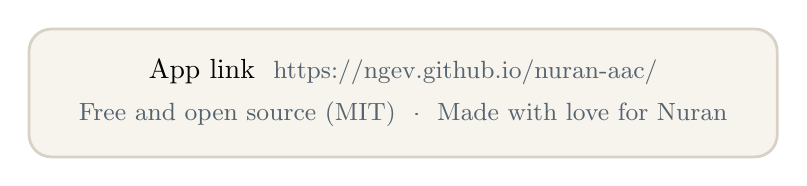
\begin{tikzpicture}
  \node[rounded corners=8pt,fill=cream,draw=linec,line width=1pt,inner xsep=18pt,inner ysep=11pt,align=center]
  {{\dispmed App link}~~\color{inksoft}\small https://ngev.github.io/nuran-aac/\\[3pt]
   \color{inksoft}\small Free and open source (MIT)~~·~~Made with love for Nuran};
\end{tikzpicture}
\end{center}

\end{document}
